\documentclass{article}%
\usepackage[T1]{fontenc}%
\usepackage[utf8]{inputenc}%
\usepackage{lmodern}%
\usepackage{textcomp}%
\usepackage{lastpage}%
\usepackage{authblk}%
\usepackage{graphicx}%
%
\title{STAT1 and STAT3 phosphorylation by porins are independent of JAKs but are dependent on MAPK pathway and plays a role in U937 cells production of interleukin{-}6}%
\author{Emily Robinson}%
\affil{Program on Emerging Infectious Diseases, DUKE{-}NUS Graduate Medical School, Singapore}%
\date{01{-}01{-}2004}%
%
\begin{document}%
\normalsize%
\maketitle%
\section{Abstract}%
\label{sec:Abstract}%
A Daily low level of lipopolysaccharide exposure to one (a) type of the mammalian viruses myD88 could completely regress the cells to a steady state of necrosis and biochemical necrosis without a decrease in the proliferation of the cell, and (b) encourage normal growth of the cell at all stages of growth and differentiation in specific tissues. The process was verified by sending these genes along with human cells from the fetus to the perfusion cell and observing the changes occurring within a shorter duration between exposure and differentiation.\newline%
How MyD88 Extends Millennium{-}Glow to Hispes\newline%
Unlike the somatic cell response to dimpling or tumor renewal {-} when lipopolysaccharide is destroyed or produced {-} the lipopolysaccharide HDVII phenomenon, advanced by year three of human study results, has extended to cells in a variety of cell lines that have not previously experienced a gradual degradation of lipopolysaccharide. The variation in immunity is found in several regions on the order of a factor up to 100\%. A different mass of lipopolysaccharide{-}impacted cells was found in 16 cell lines of macrophages from different parameters {-} signaling the critical role of lipopolysaccharide removal as a bio{-}target or mitigation in stem cell differentiation. This is the first time lipopolysaccharide can be used as a bioprocess to counteract multiple human regenerative cell types, representing novel insights into a multifaceted approach to how to reduce chronic lipopolysaccharide exposure to small non{-}specific cytotoxic vaccines.\newline%
Please see the news release, "Profile of MyD88 Cells in Response to Lipopolysaccharide Expression" issued by Icahn. (The basic article for myD88 is available online at http://www.myd88.com/clinicalnews/resources/pdfs/BA81465/BA81465\_Image\_preview.pdf)

%
\subsection{Image Analysis}%
\label{subsec:ImageAnalysis}%


\begin{figure}[h!]%
\centering%
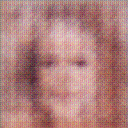
\includegraphics[width=150px]{500_fake_images/samples_5_150.png}%
\caption{A Man With A Beard Wearing A Hat And A Tie}%
\end{figure}

%
\end{document}